\FloatBarrier
\subsection{Question 2}
The required delay in the transfer function is implemented as shown in \autoref{code:sstr21}. Rest of the code remains as presented in \autoref{code:sstr11}. As shown in \autoref{fig:sstr21}, the implemented system is stable and returns to its equilibrium point at $0$. And in \autoref{fig:sstr22}, cummulative loss of the system is bounded.

\begin{code}
	\begin{matlabcode}{firstnumber = 10}
%% Transfer function
G_s = 3*(0.4*s+1)*(s+0.8)/((3*s+1)^2*(s-1))*tf(1,[1,0,0]);
	\end{matlabcode}
	\captionof{listing}{Minimum variance controller with delay}
	\label{code:sstr21}
\end{code}

\begin{figure}
	\centering
	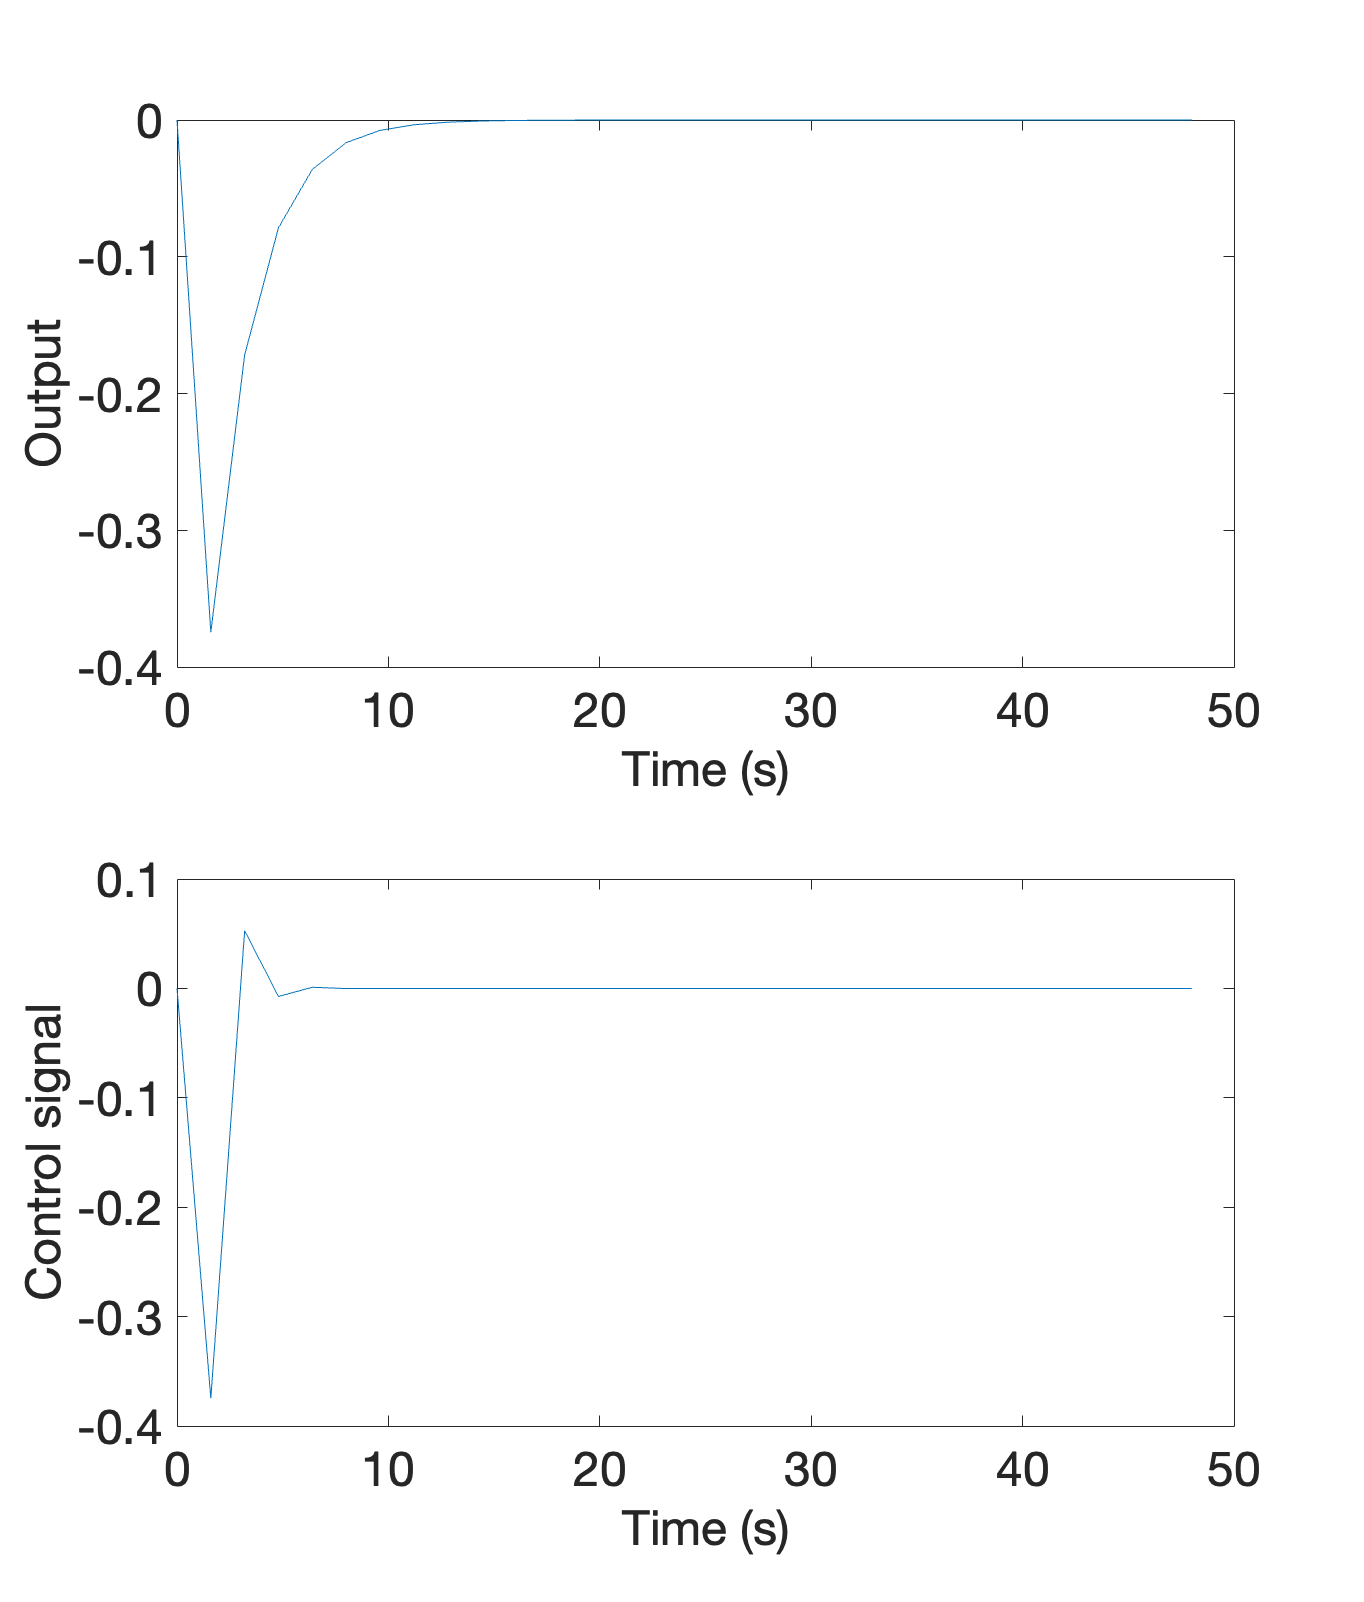
\includegraphics[width=\textwidth]{images/sstr21.png}
	\caption{Minimum variance controller with delay, output and control}
	\label{fig:sstr21}
\end{figure}

\begin{figure}
	\centering
	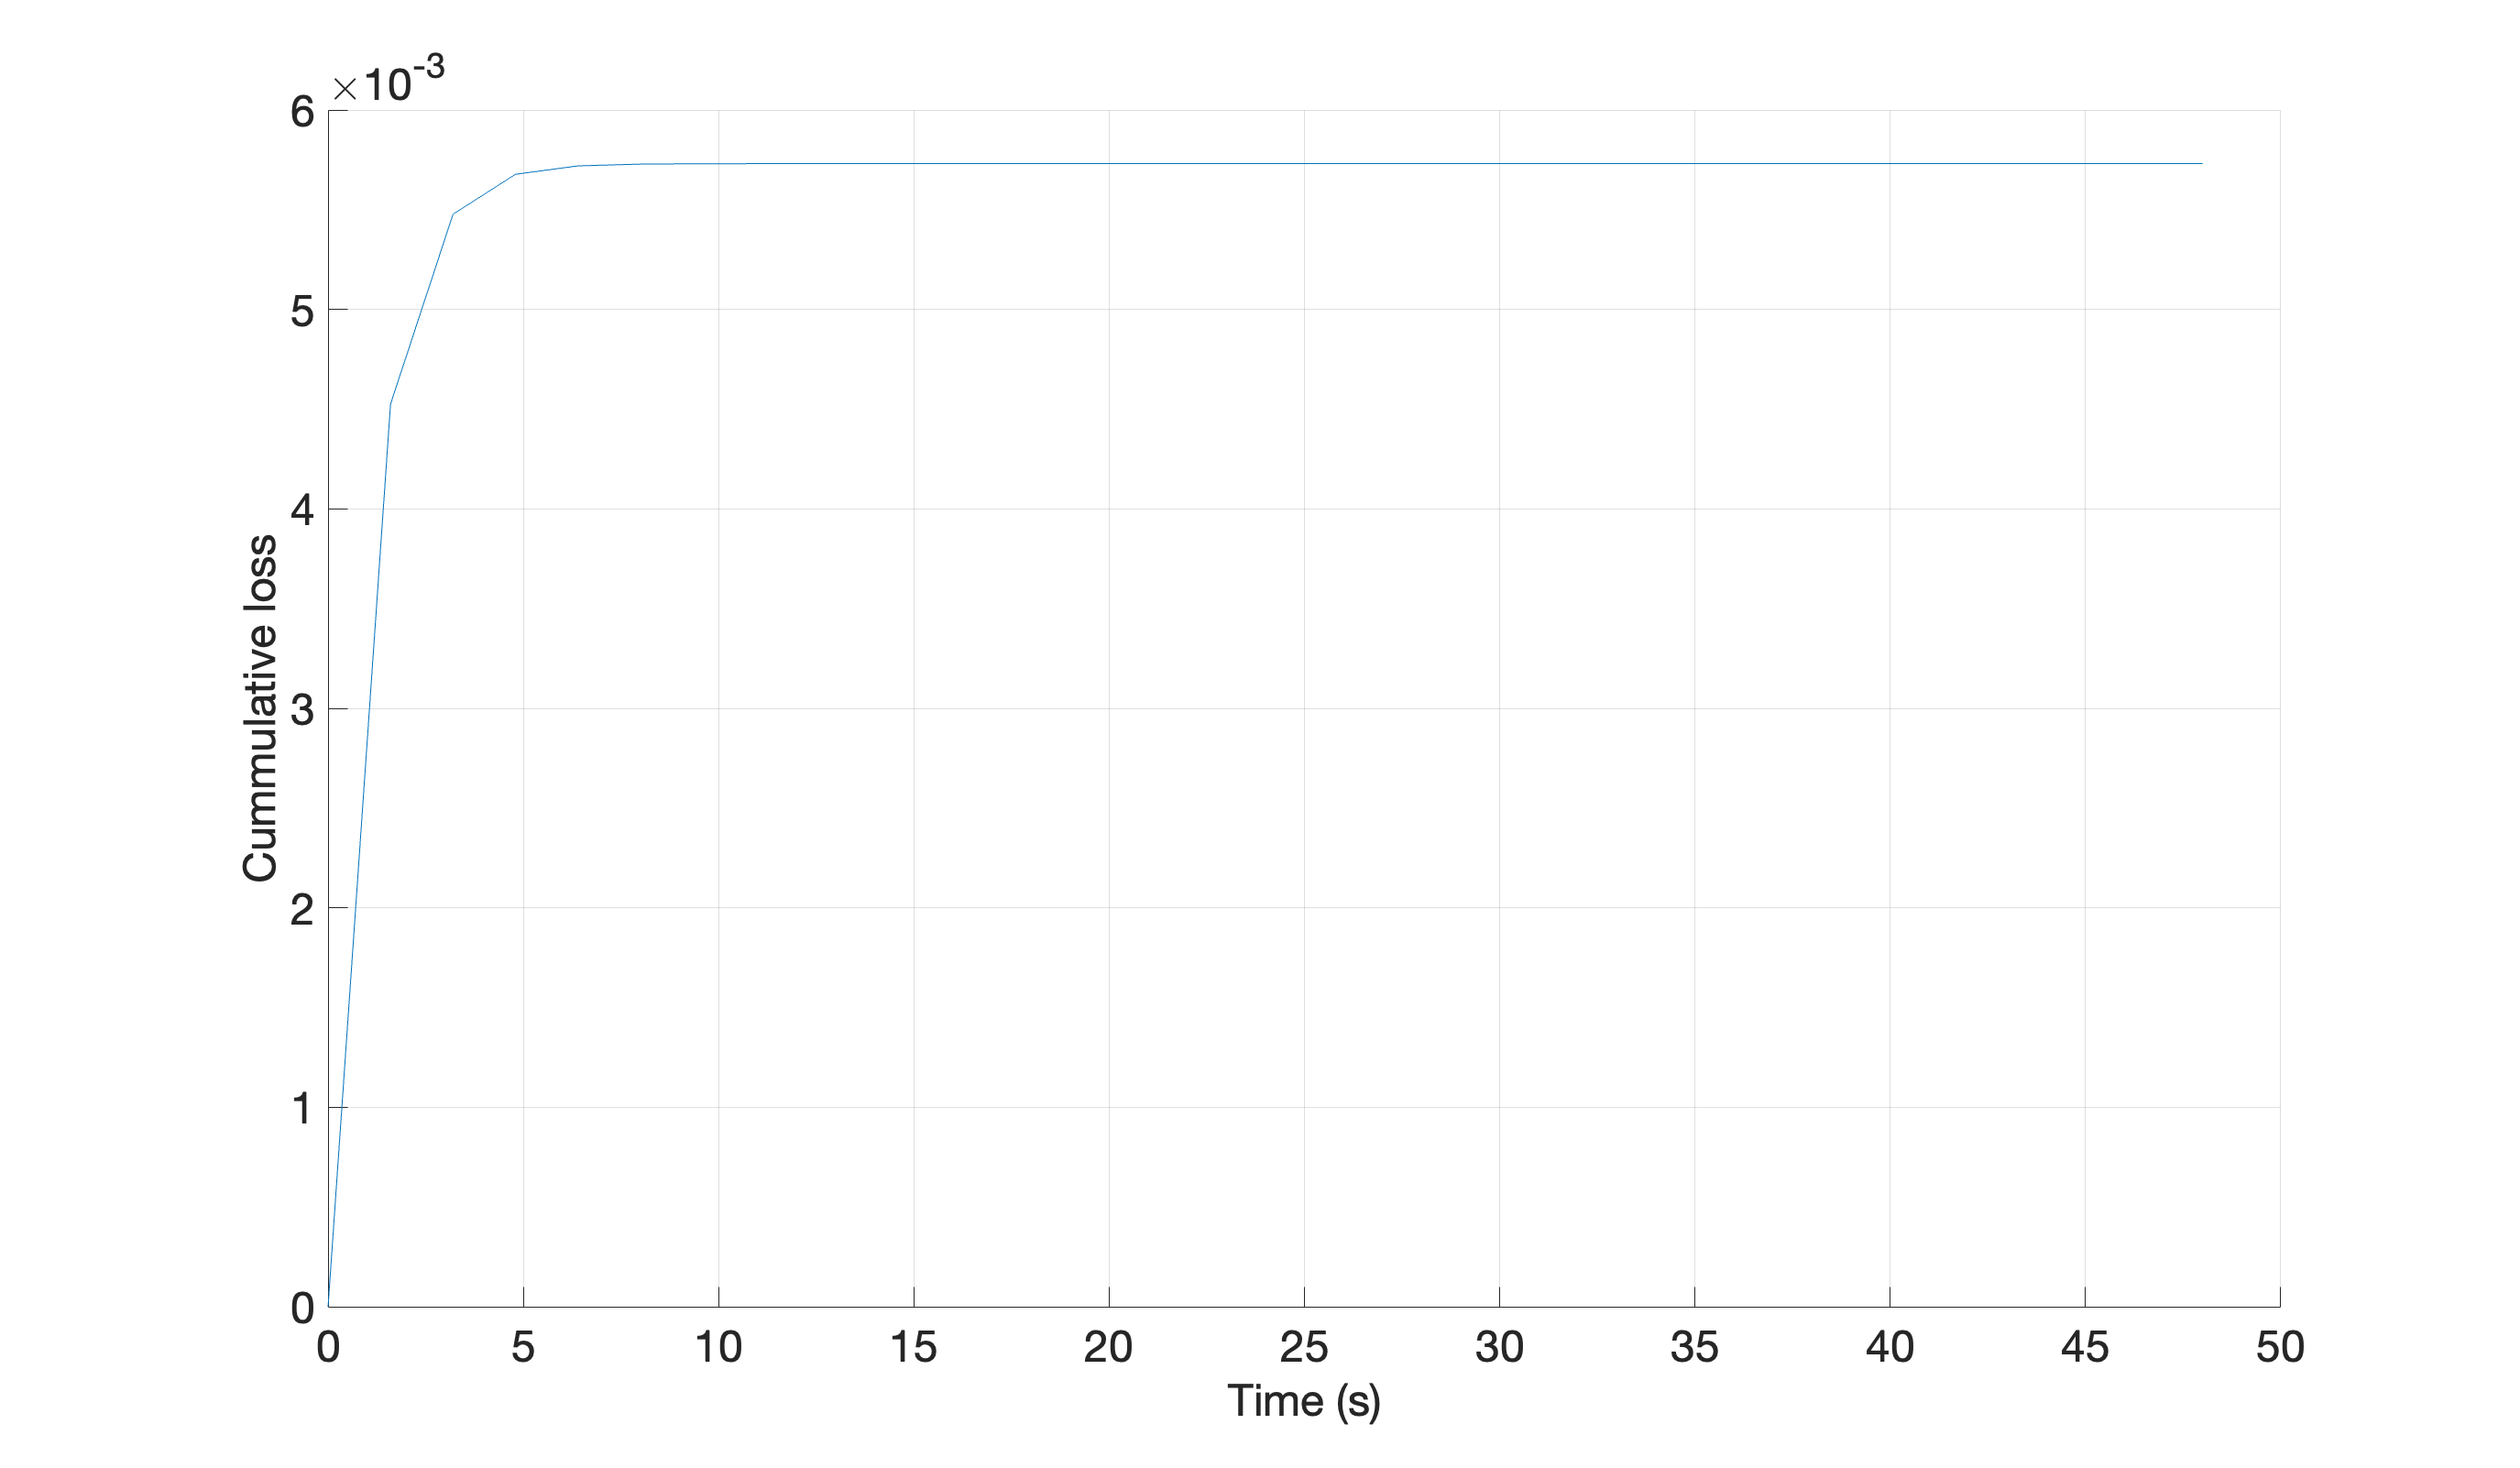
\includegraphics[width=\textwidth]{images/sstr22.png}
	\caption{Minimum variance controller with delay, cummulative loss}
	\label{fig:sstr22}
\end{figure}

\noindent The code for this section is available at \lstinline|assignment3/SSTR/SSTR_2.m|. 

